\begin{frame}\frametitle{Extended Kalman Filter (EKF)}%estimating the state of a nonlinear dynamic system
The goal is to estimate the vehicle state $\vect{X}(k)$ using sensor measurements $\vect{Z}(k)$, process $\vect{N}(k-1)$ and measurement $\vect{M}(k)$ noise. \\
\begin{columns}
	\column{.45\textwidth}
	\begin{block}{How does it work?}
	\centering
	\includegraphics[width=0.85\linewidth]{fig/diagram-kalman.pdf}
	\end{block} 
\vspace{-25pt}	
	\begin{equation*} 
	\vect{X}(k) = f(\vect{X}(k-1), \vect{N}(k-1)) \; prediction
	\end{equation*}
\vspace{-25pt}	
	\begin{equation*}
	\vect{Z}(k) = h(\vect{X}(k), \vect{M}(k))  \; measurement%= \vect{H} \vect{X}(k \mid k-1)  + \vect{M}(k)
	\end{equation*}

\column{.45\textwidth}
\vspace{-5pt}
	\begin{itemize}
		\item \begin{footnotesize}``standard'' in nonlinear estimation, \textit{Bayesian} approach\end{footnotesize} %used in other applications - GPS, nav
		%\item \begin{footnotesize}\end{footnotesize}   % involving computing posterior PDF 
		\item \begin{footnotesize}$1^{st}$ order Taylor expansion of the nonlinear functions \end{footnotesize} 
		\item \begin{footnotesize}provides estimation uncertainties in form of error covariance matrices \end{footnotesize} 
		\item \begin{footnotesize}difficult tuning \end{footnotesize}
		\item \begin{footnotesize}reliable for systems that are almost linear on the time scale of the updates \end{footnotesize}
	\end{itemize}	
	%\begin{block}{Interesting alternative: Unscented Kalman Filter}
	%\end{block}
\end{columns}
\end{frame}